% Template for Cogsci submission with R Markdown

% Stuff changed from original Markdown PLOS Template
\documentclass[10pt, letterpaper]{article}

\usepackage{cogsci}
\usepackage{pslatex}
\usepackage{float}
\usepackage{caption}

% amsmath package, useful for mathematical formulas
\usepackage{amsmath}

% amssymb package, useful for mathematical symbols
\usepackage{amssymb}

% hyperref package, useful for hyperlinks
\usepackage{hyperref}

% graphicx package, useful for including eps and pdf graphics
% include graphics with the command \includegraphics
\usepackage{graphicx}

% Sweave(-like)
\usepackage{fancyvrb}
\DefineVerbatimEnvironment{Sinput}{Verbatim}{fontshape=sl}
\DefineVerbatimEnvironment{Soutput}{Verbatim}{}
\DefineVerbatimEnvironment{Scode}{Verbatim}{fontshape=sl}
\newenvironment{Schunk}{}{}
\DefineVerbatimEnvironment{Code}{Verbatim}{}
\DefineVerbatimEnvironment{CodeInput}{Verbatim}{fontshape=sl}
\DefineVerbatimEnvironment{CodeOutput}{Verbatim}{}
\newenvironment{CodeChunk}{}{}

% cite package, to clean up citations in the main text. Do not remove.
\usepackage{cite}

\usepackage{color}

% Use doublespacing - comment out for single spacing
%\usepackage{setspace}
%\doublespacing


% % Text layout
% \topmargin 0.0cm
% \oddsidemargin 0.5cm
% \evensidemargin 0.5cm
% \textwidth 16cm
% \textheight 21cm

\title{Caregiver reconstruction of children's errors: the preservation of
complexity in language}


\author{Madeline Meyers \and Daniel Yurovsky \\
        \texttt{\{mcmeyers, yurovsky\}@uchicago.edu} \\
       Department of Psychology \\ University of Chicago}

\begin{document}

\maketitle

\begin{abstract}
Why do languages change? One possibility is they evolve due to two
competing pressures: one, for the language to be easily transmitted to
new generations---and hence simple---and another, for the language to be
a useful, descriptive form of communication---and hence more complex.
However, few studies have explored these pressures in the most skilled
language learners: children. Conventional iterated learning studies
focus on the transmission of a novel language from one adult to the
next. However, this ignores one of the important features of language
learning, namely, receiving feedback. This study compares adult
performance on a conventional iterated learning task with their
performance on a task which allows for error correction by a secondary
participant. Results show that adding this error-correcting participant
allows a greater level of complexity to be retained in the language
compared with the baseline task. Data collection is ongoing with
children, but current results suggest that editors (e.g.~parents) may be
playing a dual role in both child language acquisition and language
evolution by re-introducing complexity into a given language.

\textbf{Keywords:}
communication; language acquisition; language evolution; iterated
learning
\end{abstract}

\section{Introduction}\label{introduction}

How do you ask a group of people where they are going in Spanish? In
Spain, the answer depends on the group: you might ask ``Donde van
ustedes?'' of a group of work colleagues, but to address your friends,
you use the informal ``Donde váis vosotros?'' instead. In Mexican
Spanish, this distinction has disappeared, and the ``ustedes'' form is
used exclusively. Why did Spanish change in this way, simplifying and
shedding the formal second person plural? Why do languages change at
all, aside from acquiring new vocabulary? One working theory is that
languages evolve, like biological organisms, to adapt to two dynamic
competing pressures: one, to be easily transmitted and learned (and
hence simple), and another, to be an effective system for communication
(and hence informative)(Lupyan \& Dale, 2010).

Children are often the actors who drive language evolution (Senghas,
2003), yet they differ from adults in their 1) cognitive capabilities,
namely, memory systems (Kempe, Gauvrit, \& Forsyth, 2015), 2) interests
and early vocabularies, and 3) conversation partners. Therefore, though
children are skilled language learners, their developing cognitive
systems prevent aspects of language that are difficult to learn and
remember from being passed on---pushing languages towards simplicity
(Hudson Kam \& Newport, 2005; Senghas, 2003). But, languages that become
too simple can lose the ability to be effective for communication
(Kirby, Griffiths, \& Smith, 2014). What enables languages to retain
their communicative utility in the face of these learnability pressures?

The following study tests a novel hypothesis for the maintenance of
structure in language: Communicative inference by caregivers. Children's
language learning is greatly influenced by those around them--especially
their caregivers. These caregivers determine the majority of their
child's language input, and are responsible for seeing that their
children develop effective and useful systems of communication. Even the
youngest children are not passive learners of language---they are active
participants, engaging in conversations with their parents. These adults
are experts both in the language and in the children themselves---they
understand the child's intuitions, personality, and context. Caregivers
play an important interpretive role in these interactions by their
ability to understand the intended target of children's errorful
productions (Chouinard \& Clark, 2003). They may reconstruct their
child's language in numerous ways-- through explicit or implicit
correction, or simply through modeling correct use of the language over
time (Hudson Kam \& Newport, 2005). These reconstructions may be a
mechanism by which more structure is retained in language than children
could sustain alone.

\subsection{Using iterated learning to study language
change}\label{using-iterated-learning-to-study-language-change}

\begin{CodeChunk}
\begin{figure}[tb]

{\centering 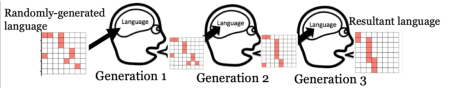
\includegraphics{figs/ill_outline-1} 

}

\caption[In the standard iterated learning paradigm, each participant is trained on input from the previous participant, creating a chain of generational transmission replete with implicit learning errors]{In the standard iterated learning paradigm, each participant is trained on input from the previous participant, creating a chain of generational transmission replete with implicit learning errors.}\label{fig:ill_outline}
\end{figure}
\end{CodeChunk}

One way to study language acquisition in the lab is to use the iterated
learning paradigm. Created to study the effects of simplicity and
informativity on inter-generational language evolution, this method is
useful for testing the proposed hypotheses (Kirby et al., 2014). In an
iterated learning paradigm, one participant is trained on a
randomly-generated language---for example, a set of words created by
arbitrarily pairing syllables together. The participant is later asked
to recall the language, and their responses are given as training input
for the next subject, thus creating a transmission chain (see Figure 1).
This iterated process mimics the transmission of language across
generations, with each participant unintentionally changing the language
through their memory biases. Few iterated learning studies, however,
have used children as research subjects. A study by Kempe et al. (2015)
compared child (5-8) and adult performances on an iterated learning task
using a novel dot-pattern paradigm (showed in Figure 1). Their results
found that structure emerged faster in children than adults---that is,
the children's patterns simplified much faster than the adult's,
allowing them to be easier to reproduce earlier in the transmission
chain. This study provides evidence of the importance of looking at both
children and adults in an iterated learning paradigm, as they have
different cognitive skills which affect their performance in
language-learning tasks (Kempe et al., 2015). However, language
evolution can never be fully grasped using this paradigm with only
separate adult or child earning chains, because language learning does
not occur only within the same age group (horizontal transmission), or
only across age groups (vertical transmission), but it occurs
dynamically, in both directions. In a true language-acquisition
situation, a child receives both language input and feedback from their
caregiver and uses it to interact with their peers throughout life,
eventually growing into a new teacher-caregiver.

The following study uses a diffusion chain paradigm with an adaptation
of Kempe et al. (2015)'s original non-linguistic task to investigate how
the pressures of descriptiveness and transmissibility operate in adults
when their responses are subject to error correction by a secondary
participant. We hypothesize that these error-correctors (e.g., parents
and teachers) are pivotal not only to an individual child's successful
language acquisition, but also to the evoulution of a language as a
whole. This is because those who correct mistakes and provide feedback
are able to protect against the transmissibility (simplicity) bias,
which is likely stronger in early language learners, by re-introuding
and preserving complexity in language.

\section{Methods}\label{methods}

In a baseline experiment, adults participated in a standard iterated
learning study, using stimuli adapted from Kempe et al. (2015).
Participants were told to reproduce patterns on grids, and each user's
responses were used as training input for the subsequent participant. In
the second, dyad experiment, the first participant was designated as a
``learner'', and completed the same task as in the baseline experiment.
A secondary participant--the ``fixer''--was given an adjusted task,
where instead of reproducing a pattern on a grid, they were told to
``fix the errors'' on a grid pattern, in order to match the same target
pattern. The fixer's responses were passed as target input for the
subsequent learner.

The experimental task was designed online using JavaScript, HTML, and
CSS, and was hosted as a web page accessed through a server. All adult
data was collected through Amazon Mechanical Turk, an online
crowdsourcing cite commonly used in psych studies (Buhrmester, Kwang, \&
Gosling, 2011). Participants were compensated with \$0.50 for their
participation.

In order to store user's responses to be accesed by the next participant
in a transmission chain, data was stored using Google Sheets, and
accessed during the task using an API.

Subjects in the baseline condition and ``learners'' in the dyad
condition were told that in this task, they would be re-creating
patterns on a grid. After a consent screen, subjects first viewed a
training trial with two 8x8 grids on the screen -- a target grid, with
10 cells colored in and a blank grid. They were told to make the blank
grid match the target grid exactly, and were unable to progress until
the grids matched exactly. Following this trial, participants were
informed that they would see a target grid appear on the screen for 10
seconds, followed by a picture (a visual mask) displayed for 3 seconds.
After the visual mask, participants viewed a blank 8x8 grid where they
were given 60 seconds to re-create the target grid. Subjects could click
on any cell in the grid to have it change color, and could also remove
any block which they placed. On the input grid screen, there was a
counter that varied based on the number of blocks a participant had
placed in order to help the subject place exactly 10 blocks, as well as
a timer. Subjects had 60 seconds to complete each trial, and an audio
cue reminded them when they had only 20 seconds left to complete their
pattern. There were additional audio cues such as sparkling sounds,
encouragement, etc. throughout the task. After 3 practice trials,
participants were told that the study would begin. The subject's
performance on the practice trials was used as an attention check to
determine whether their data would be passed to the next participant. If
the subject scored less than 75\% accuracy on the last 2/3 scored
practice trials, their data would be marked as ``unavailable'' to the
next user in the chain. There were 6 experimental trials, where
participants viewed either the randomly-generated grids or the grids
passed from a previous participant in the chain, rather than the simpler
practice target grids. Participants were required to select 10 targets
before moving to the next trial; if the participant failed to select 10
items before time ran out on an experimental trial, their data was
removed from the study. Approximately 7\% (n=38) of participants in the
baseline condition and approximately 7\% (n=78) of participants in the
dyad condition were excluded from analysis due to failure to meet
accuracy requirements on the practice trials or failure to select 10
blocks on one or more experimental trials.

Those in the ``fixer'' condition in the dyad experiment were given an
adapted task. The only difference was that throughout the study, they
were not told to re-create the target grid, but to fix a grid they saw
to make it resemble the target grid exactly. Essentially, fixers in the
dyad condition viewed the same target grid as the learners, but instead
of seeing a blank input grid, they saw a grid that already had 10
elements filled in -- the elements that the previous learner had
submitted. The participant could then click and unclick the elements and
change their positions. There was no ``reset'' button on these input
grids, so they reflect participants first memory instincts.

Transmission chains consisted of 12 generations each, and 40 separate
chains were run during each condition of the study. Each chain began
with the same initial target grid. The participant in the first
generation received the initial grid as their target, and each
subsequent generation received the previous generation's inputs as their
targets. In the dyad condition, a generation consisted of a learner, who
re-created the target grid, and a fixer, who received the same target
grid as well as the learner's input grid as their grid to edit. The
fixer's final input was used as the target grid for the subsequent
generation.

The initial 8x8 grids were generated randomly. Each cell filled in
corresponded to a number which was generated using Excel's random number
generator. A random number 1-64 was assigned to each cell in the grid,
and the 10 random numbers generated for each of the 6 practice trials
determined the pattern viewed by participants in the first generation.
The 6 grid patterns which began the iteration all had initial similar
transmission accuracy, so there is reason to believe that none of the
initial patterns were easier or harder to acquire, all had initial
accuracies of approximately 55\%. All initial patterns remained constant
across all chains and conditions of the study; this allows a consistent
comparison of aggregate data. Aside from the first practice trial, where
participants were required to reproduce perfectly, participants never
received feedback on their responses.

\subsection{Analysis}\label{analysis}

\subsubsection{Percent Accuracy}\label{percent-accuracy}

Percent accuracy was calculated as the proportion of targets (out of 10)
which were placed in the same location on the target and input grids.
This measure does not account for the degree of error for targets placed
in incorrect locations.

\subsubsection{Complexity}\label{complexity}

To calculate the complexity of the grid patterns produced, we used three
measures: algorithmic complexity, chunking, and edge length. All
analysis code was adapted from Gauvrit, Soler-Toscano, \& Guida (2017).
Algorithmic complexity is calculated using the Block Decomposition
Method, a measure of Kolmogorov-Chaitin Complexity applied to
2-dimensional patterns (Zenil, Soler-Toscano, Dingle, \& Louis, 2014).
Essentially, BDM uses the coding theorem method to break each two-color
8x8 grid into 4x4 patterns. If each 4x4 pattern is p, the formula for
computing BDM is Sum p (log2(np) + K(p)) (Kempe et al., 2015). Here,
K(p), or the complexity of a 4x4 pattern, is defined as the length of
the program taken as input by a Turing machine, and nP is the frequency
of each pattern p (Zenil, Soler-Toscano, Delahaye, \& Gauvrit, 2015).
This measure of complexity accounts for the shortcomings of other
complexity measures such as entropy, as it accounts for the condition
where a checkerboard pattern is not probable, yet is not typically
defined as complex. In this case, BDM would see this pattern as having a
lower complexity than a different randomly-generated pattern.

Chunking is the number of groups of colored blocks which share an edge.
The more groups of blocks, the easier the pattern is to transmit, and
the lower the complexity is. Edge length is the total perimeter of the
colored blocks. If all blocks were in one chunk, the edge length would
be low, and the complexity of the pattern would likely be lower compared
to if none of the chosen targets shared an edge (Gauvrit et al., 2017).

\section{Results}\label{results}

\subsection{Baseline Experiment}\label{baseline-experiment}

\subsection{Dyad Experiment}\label{dyad-experiment}

\begin{CodeChunk}
\begin{figure}[tb]

{\centering 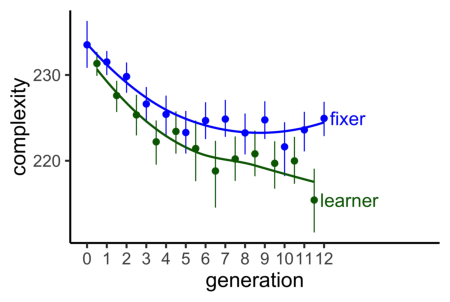
\includegraphics{figs/dyad_complexity-1} 

}

\caption[Fixers reintroudce complexity which is lost by learners in the dyad condition]{Fixers reintroudce complexity which is lost by learners in the dyad condition.}\label{fig:dyad_complexity}
\end{figure}
\end{CodeChunk}

\begin{CodeChunk}
\begin{figure}[tb]

{\centering 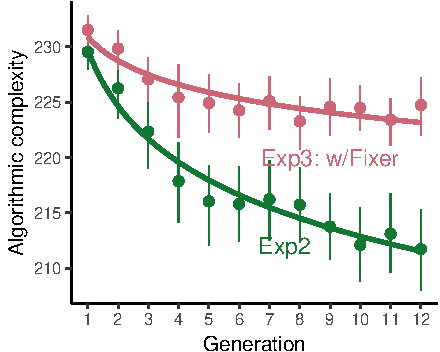
\includegraphics{figs/both_complexity-1} 

}

\caption[The presence of a fixer in the dyad condition causes a much greater level of complexity to be retained across the evolution of a novel language]{The presence of a fixer in the dyad condition causes a much greater level of complexity to be retained across the evolution of a novel language.}\label{fig:both_complexity}
\end{figure}
\end{CodeChunk}

\section{Discussion}\label{discussion}

Although this is a non-linguistic task,

\section{Future Directions}\label{future-directions}

Data collection is ongoing with children ages 6-8 at the Museum of
Science and Industry in Hyde Park, Chicago. Children are participants in
the baseline task, and are learners in the dyad task, with mTurkers as
the fixers. Children complete the task on an iPad, and receive their
choice of stickers as compensation. iPad tasks have many advantages over
other research methods, including the paper-and-sticker task used by
Kempe et al. (2015) because the use of an iPad reduces the completion
time of the study and is engaging for young children Frank, Sugarman,
Horowitz, Lewis, \& Yurovsky (2016). Parents of the children in the
study completed an additional child information sheet about the child's
language experiences and home environment. We expect to see similar
trends in complexity over time with children as were seen with adults,
namely, in the dyad task, adults reintroduce complexity which is lost by
child language learners. However, we expect sharper initial decreases in
complexity with children, in line with the findings of Kempe et al.
(2015). We plan to conduct a set of qualitative analyses on the patterns
produced by adults and children, in order to see whether children are
simply making more errors than adults, or if they are making
fundamentally different errors, perhaps reflecting their differential
language-learning systems.

\vspace{1em}
\fbox{\parbox[b][][c]{7.3cm}{\centering All code for these analyses are available at\ \url{https://github.com/mcmeyers/iteratedlearning}}}

\section{Acknowledgements}\label{acknowledgements}

This research was funded by a James S. McDonnell Foundation Scholar
Award to DY.

\section{References}\label{references}

\setlength{\parindent}{-0.1in} \setlength{\leftskip}{0.125in}

\noindent

\hypertarget{refs}{}
\hypertarget{ref-buhrmester-2011}{}
Buhrmester, M., Kwang, T., \& Gosling, S. D. (2011). Amazon's mechanical
turk: A new source of inexpensive, yet high-quality, data?
\emph{Perspectives on Psychological Science}, \emph{6}(1), 3--5.

\hypertarget{ref-chouinard-2003}{}
Chouinard, M. M., \& Clark, E. V. (2003). Adult reformulations of child
errors as negative evidence. \emph{Journal of Child Language},
\emph{30}(3), 637--669.

\hypertarget{ref-frank-2016}{}
Frank, M. C., Sugarman, E., Horowitz, A. C., Lewis, M. L., \& Yurovsky,
D. (2016). Using tablets to collect data from young children.
\emph{Journal of Cognition and Development}, \emph{17}(1), 1--17.

\hypertarget{ref-gauvrit-2017}{}
Gauvrit, N., Soler-Toscano, F., \& Guida, A. (2017). A preference for
some types of complexity comment on ``perceived beauty of random texture
patterns: A preference for complexity''. \emph{Acta Psychologica},
\emph{174}, 48--53.

\hypertarget{ref-hudsonkam-2005}{}
Hudson Kam, C. L., \& Newport, E. L. (2005). Regularizing unpredictable
variation: The roles of adult and child learners in languagae formation
and change. \emph{Language Learning and Development}, \emph{1}(2),
151--195.

\hypertarget{ref-kempe-2015}{}
Kempe, V., Gauvrit, N., \& Forsyth, D. (2015). Structure emerges faster
during cultural transmission in children than in adults.
\emph{Cognition}, \emph{136}, 247--254.

\hypertarget{ref-kirby-2014}{}
Kirby, S., Griffiths, T., \& Smith, K. (2014). Iterated learning and the
evolution of language. \emph{Current Opinion in Neurobiology},
\emph{28}, 108--114.

\hypertarget{ref-lupyan-2010}{}
Lupyan, G., \& Dale, R. (2010). Language structure is partly determined
by social structure. \emph{PLoS ONE}, \emph{5}(1), 1--10.

\hypertarget{ref-senghas-2003}{}
Senghas, A. (2003). Intergenerational influence and ontogenetic
development in the emergence of spatial grammar in nicaraguan sign
language. \emph{Cognitive Development}, \emph{18}, 511--531.

\hypertarget{ref-zenil-2015}{}
Zenil, H., Soler-Toscano, F., Delahaye, J.-P., \& Gauvrit, N. (2015).
Two-dimensional kolmogorov complexity and an empirical validation of the
coding theorem method by compressibility. \emph{PeerJ Computer Science},
\emph{e23}.

\hypertarget{ref-zenil-2014}{}
Zenil, H., Soler-Toscano, F., Dingle, K., \& Louis, A. A. (2014).
Correlation of automorphism group size and topolical properties with
program-size complexity evaluations of graphs and complex networks.
\emph{Physica A}, \emph{404}, 341--358.

\end{document}
